\section{Theoretical studies of electrolytes for metal-ion batteries}

In parallel to experimental works, research on electrolytes was supported by numerous computational studies. Recent reviews provide general information about the theoretical modeling of electrolytes for LIBs~\cite{li-modeling-review} and non-lithium ionic batteries~\cite{na-modeling-review}. In this chapter some selected examples will be described in more detail.

\subsection{Lithium Ion Batteries}

The first big group of studies involve quantum chemical (QC) methods. For systems based on organic carbonates, calculations for Li$^{+}$-solvent pairs in the gas phase were performed with Density Functional Theory (DFT) methods. They indicated the preferred lithium coordination number in the complex with EC~\cite{li-ec-dft,li-diffusion-dft-aimd} and optimized structures of complexes with EC and PC~\cite{li-ec-pc-dft}. A similar study was carried out for LiClO$_4$ solutions in EC and PC~\cite{li-dft-clo4}. For these systems theoretical Raman spectra obtained from DFT calculations in the gas phase were also used to determine the extent of cation-solvent interactions in the solvation shell~\cite{li-raman-ec-dft}. Other DFT calculations performed for systems with LiPF$_6$ dissolved in a~series of organic carbonates identified EC as the solvent with the strongest coordination ability for both the cation and the anion~\cite{li-pf6-dft}. In a~study investigating associates of carbonates and lithium ions, the analysis of intermolecular O-Li-O interactions~\cite{li-dft-associations}, led to the conclusion that the Li-O interaction behaves as ionic. The simplest computational methods investigate systems in vacuum. Nevertheless, for proper modeling of the electrolytes and solutions, inclusion of solvent effects is necessary. The cost-effective method is to apply an implicit solvent method, e.g.~the Polarizable Continuum Model (PCM). The use of continuum solvation models for interactions in electrolytes was studied in several works~\cite{pcm-1,lib-solvent-effects,pcm-2}. Example of obtained complexes for LiClO$_4$ in diglyme are presented in Figure~\ref{fig:introduction-li-clo4-diglyme}. More advanced modeling may involve explicit solvent model or hybrid (continuous-explicit) approaches~\cite{pcm-3,pcm-4}. DFT with implicit solvent methods were used for determination of oxidative~\cite{li-dft-oxidative} or reductive~\cite{li-dft-reductive,li-dft-md-reductive} solvent decomposition mechanisms. Electronic structure calculations for several lithium salts were performed at the DFT level with the PCM approach~\cite{lib-solvent-effects}. Another study shows DFT results for the binding energy between lithium cations and glymes with increasing chain length~\cite{li-glyme-dft}.

QC calculations were also applied to study the ILs and salt solutions in ILs. Three systems of big cation-anion clusters for EMIM-BF$_4$, EMIM-PF$_6$ and EMIM-TFSI were modeled by DFT~\cite{li-il-dft-1}. Another work involved DFT calculations for ionic aggregates responsible for the conductivity of the electrolyte~\cite{li-il-dft-2}. DFT was also used to determine the electrochemical stability window for ILs based on imidazolium derivatives~\cite{li-il-stability-window-dft}. IR spectra obtained from DFT calculations helped to analyze the changes of TFSI$^{-}$ anion vibrations resulting from the interaction with lithium~\cite{lib-vibrational-modeling}.

QC methodology was shown a~useful tool to model small molecules or aggregates. However, to properly describe condensed-phase systems, such as solutions, implicit methods like PCM are insufficient. For that purpose, molecular dynamics (MD) methods are used because they allow to explicitly describe solvent effects, to study the structure changes over time and to calculate important parameters of electrolytes: viscosity, diffusion coefficients, and conductivity. For ILs, in which electrostatic interactions are crucial, in classical force field (FF) MD one of the issues is including polarizability in the FF. Classical FFs such as OPLS~\cite{ff-opls} or Lopes/P\'{a}dua~\cite{ff-lopes-padua} are non-polarizable, that is, do not include induced dipole moments in the evaluation of the electrostatic contribution to energy. However, it was shown that polarization effects are significant for electrolytes~\cite{borodin-old-1,borodin-old-2}, and become particularly important for ILs~\cite{ff-polarizability,na-dft-5}. The two main approaches to model polarization are to explicitly calculate induced dipoles (such as in the FF APPLE\&P~\cite{ff-applep}) or to effectively simulate them via Drude oscillators~\cite{ff-drude}. The latter method was used to develop a~polarizable version of Lopes/P\'{a}dua FF for ILs~\cite{ff-lopes-padua-polarizable}. Another possible method to include polarization is the scaling of the charges of ionized groups~\cite{ff-scaling-charges}. In general, in polarizable FFs, calculated viscosity is smaller and conductivity larger than in non-polarizable FF, respectively~\cite{ff-lopes-padua-polarizable}. The constantly growing computational power of modern computers leads to increased applications of ab initio molecular dynamics (AIMD)~\cite{aimd-perspectives-1,aimd-perspectives-2,aimd-perspectives-3}.

\begin{figure}[ht]
    \centering
    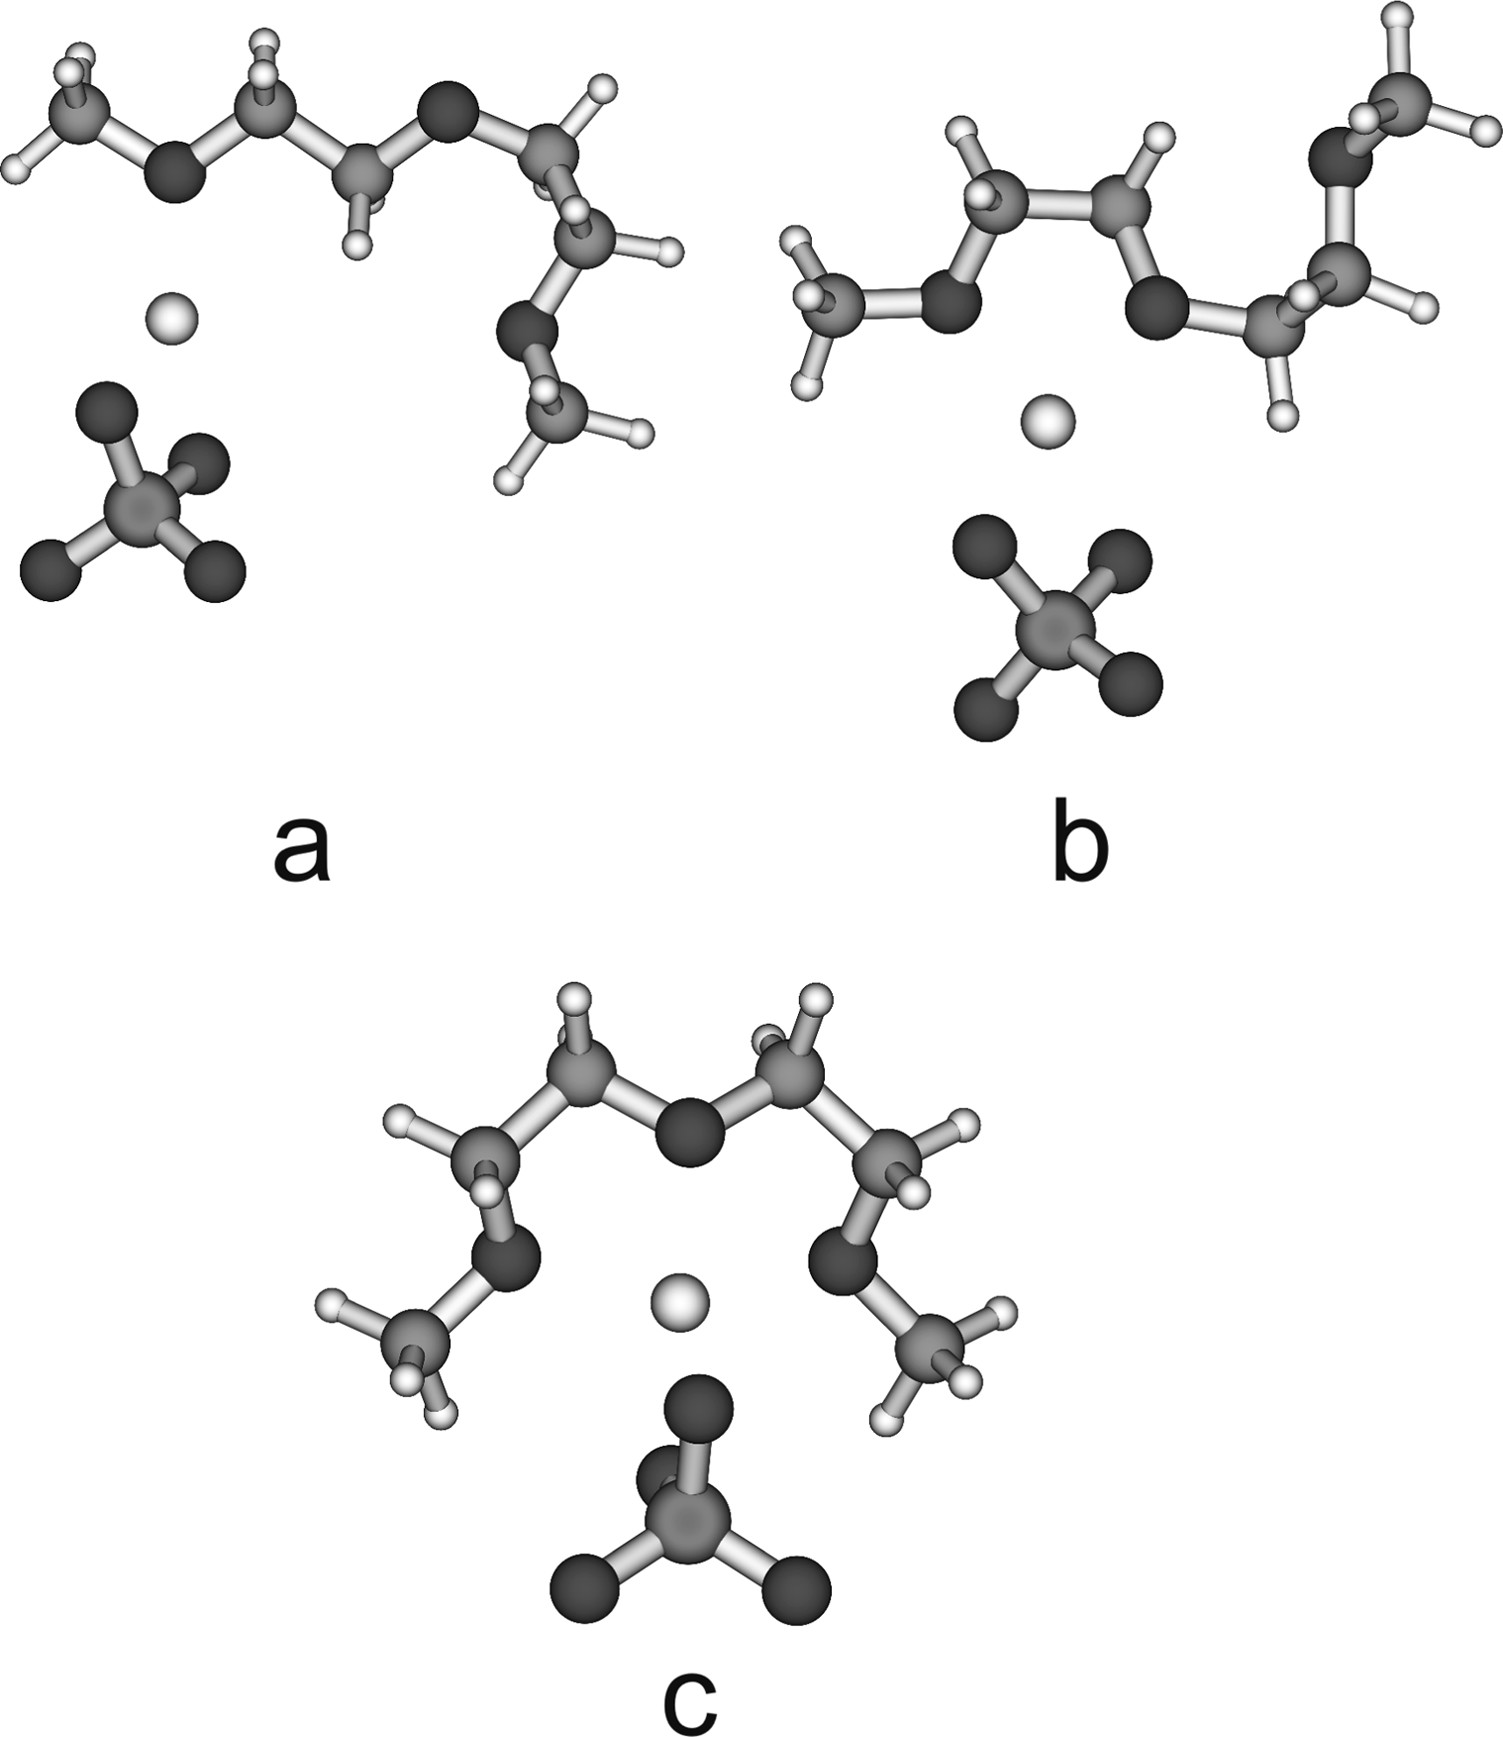
\includegraphics[width=0.5\textwidth]{img/1-introduction/li-clo4-diglyme.png}
    \caption{Structures of diglyme-LiClO$_4$ complexes calculated with DFT methods~\cite{pcm-2}}
    \label{fig:introduction-li-clo4-diglyme}
\end{figure}

MD simulations were conducted for several systems relevant to LIB electrolytes. MD with polarizable force field (PFF) was performed for solid electrolyte interphase components (SEI). The results of these MD simulations allowed to determine the coordination numbers of lithium cations and calculate the conductivities of the systems~\cite{li-md-1,li-md-13}. A~similar study on the charge transport mechanism was performed for LiTFSI in PEO~\cite{li-md-2,li-md-15} or salts with PF$_6^{-}$ anion and cations based on imidazolium derivatives dissolved in PEO~\cite{li-md-3}. Other research examined the influence of the Lewis acid centers (boron or aluminum) in the electrolyte containing PEO and LiClO$_4$ on structural properties, as well as on diffusion coefficients and conductivity~\cite{li-md-16}. An approach using both QC and MD results was used to model the cation solvation shell and to predict the transport properties in liquid solutions of LiPF$_6$ in EC and its derivatives~\cite{li-md-6,li-md-11,li-diffusion-dft-aimd}. For pure, binary and ternary mixtures of PC, EC, and DMC classical MD confirmed the results of QC calculations that complexes with four solvent molecules around the lithium cation are the most stable and also revealed the existence of structural heterogeneities beyond the first coordination shell~\cite{li-md-10}. MD was also used to model the structure of the near-electrode layer depending on the electrode potential~\cite{li-md-12}. In addition, AIMD were used in lithium-based electrolyte studies, for example to determine the structural properties of LiPF$_6$ dissolved in carbonate solvents and to establish the relation between the structure of the liquid and the experimental Raman spectrum~\cite{li-md-17}. In other research, MD simulations were used to detect the mechanism of lithium ion transport in two ILs and to compare their performance in terms of conductivity~\cite{li-md-14}. To improve the results of classical MD, some specific PFFs for IL modeling were developed~\cite{li-md-4,li-md-5,li-md-7,li-md-8,li-md-9}. 

ILs were studied by MD methods not only as solvents but also as neat liquids. Classical MD was used to determine the shape of the EMIM-TFSI droplet formed in the presence of the applied electric field~\cite{il-md-2}. It was also used in determining the structure of the IL based on radial distribution functions (RDFs) and for comparison with experimental data for a~set of different ILs with cations based on imidazolium or aliphatic amines and anions including acetates, TFSI$^{-}$ and PF$_6^{-}$~\cite{il-md-10}. A~similar study was performed for ILs based on amino acid anions~\cite{il-md-11}. Other research concentrated on studying the properties of the surface between two mixtures: one consisting of water and IL and the second consisting of nonane and IL~\cite{il-md-12}. AIMD was utilized to determine the structural properties of EMIM-SCN and EMIM-Cl ILs~\cite{il-md-1}. In particular, AIMD was used to study hydrogen bonds (HBs) in gas phase and crystalline alkylammonium based ILs~\cite{il-md-7}. In another study, the structural and dynamical properties of imidazolium based ILs were studied by classical MD and compared with AIMD~\cite{il-md-9}.

The issue of applicability of the mentioned computational methods for modeling of IL systems was also discussed. Comparison between the results obtained from MP2 and from a~set of different DFT functionals~\cite{bench-ks-vs-mp2,bench-dft-vs-ai} showed that only new generations functionals such as M05-2X or KMLYP give results close to the MP2 reference. However, including the Grimme's dispersion correction~\cite{grimme-d3} improves the quality of the results, probably because of the cancelation of errors~\cite{bench-dft-grimme}. For some IL systems, DFTB was presented as a~reasonable method to speed-up calculations with acceptable loss of accuracy~\cite{bench-dftb}.

\subsection{Beyond lithium}

The biggest number of research results devoted to "beyond lithium" systems was published for liquid sodium-based electrolytes; the theoretical approaches used are basically the same as for lithium counterparts. The reduction reactions of popular carbonate solvents (EC, PC) and fluorinated EC were studied using DFT methods~\cite{na-dft-1,na-dft-2}. Other works utilized DFT for studying cation-anion interaction for both lithium and sodium cations with anions among which were FSI$^{-}$, F$^{-}$, BF$_4^{-}$ and shown that for sodium the strength of the interaction is lower than for lithium~\cite{na-dft-3,na-dft-4}. A~similar behavior was observed for sodium salt with 2,5,8,11-tetraoxatridecan-13-oate (TOTO)~\cite{na-dft-5}, which in addition is an~IL itself. For nitrile-based sodium salts, DFT was used to calculate ion-ion interaction energies and anion oxidation potentials~\cite{na-dft-6}. Other theoretical works describe the calculation of the solvation energy by DFT for about~30 common solvents for sodium batteries~\cite{na-dft-7,na-dft-8}. Different approaches to solvation effects were presented in~\cite{na-dft-9}, in which the structures for the DFT calculations were extracted from MD simulations. Another work focusing on the determination of the interaction strength describes the comparison of lithium and sodium complexes with crown ethers~\cite{na-dft-10}. DFT study of NaTFSI in imidazolium-based ILs with TFSI$^{-}$ anion showed that coordination numbers for sodium are close to~3, what is bigger than typical value of~2 obtained for the lithium analog~\cite{na-il-5}. Glyme-based systems were also studied with the use of DFT, in~\cite{na-dft-13} the oxidative stability of pentaglyme and its complex with NaTFSI was determined with the Hartree-Fock method and compared with results for different cations (Li and~K)~\cite{na-dft-14}. MP2 method was used to study the interaction energies in a~series of glymes from monoglyme to pentaglyme~\cite{na-dft-15,vibrational-exp-2,na-dft-16}. Similarly as for the lithium-based systems, polymer electrolytes were also studied. Starting with small models, the geometries of complexes between sodium and oligoglymes simulating parts of PEO were determined with HF or DFT methods~\cite{na-dft-17,na-dft-18,na-dft-19}. Other works extended this approach and also included the influence of the presence of anion in the system to determine the dependence of vibrational frequencies on the local electronic structure~\cite{na-dft-20,na-dft-21,na-dft-22,na-dft-23}. DFT methods were also utilized to study the properties of magnesium-based systems. Such works involve determination of structures of Mg-Cl complexes in tetrahydrofuran and glymes~\cite{mg-dft-1}, studies of the stability of complexes with different anions and solvents --- DMSO~\cite{mg-dft-2} and glymes~\cite{mg-dft-3}. Using DFT methodology, the thermal and electrochemical stability of complex between Mg(TFSI)$_2$ and tetraglyme were studied~\cite{na-dft-15}. The reductive stability of the complexes for Mg (TFSI)$_2$ in diglyme was studied by DFT methods~\cite{mg-dft-5}. Another usage of DFT methods included determination of bond dissociation energies, electrochemical stability window, and hydrolytic enthalpy for various mutations of the TFSI anion salts~\cite{mg-dft-6}.

Likewise lithium-based electrolytes, also for systems with sodium or magnesium DFT was used in studying the spectroscopic properties of these systems. For several carbonate solvents, including EC, PC, DMC, and DME, shifts of the Raman active ring breathing vibration and of the IR active C=O stretching vibration were reproduced~\cite{na-dft-9,vibrational-exp-3,na-dft-11}. The calculated values of the frequency shifts were lower than for the lithium analogs, due to the lower interaction energy, and were in the range between~5 and~50~cm$^{-1}$. Another example are DFT calculations of Raman spectral data for the tetraglyme and pentaglyme with NaTFSI~\cite{na-dft-12}. The calculated structural data for systems with Mg(TFSI)$_2$ and di- or triglyme were related to the experimentally measured IR spectrum~\cite{mg-dft-4}.

Sodium-based electrolytes were also studied by MD simulations. Several of these works focused on the determination of the coordination numbers of sodium cations in different solvents, carbonates~\cite{na-md-1,na-md-6}, acetonitryle~\cite{na-md-2,na-md-5} (including complexes with crown ethers~\cite{na-md-4}) and DMSO~\cite{na-md-3}. They showed that the coordination numbers for Na$^{+}$ are usually in the range of 5-7, except for linear carbonates, where they are lower and close to~3. Another study examined the properties of the SEI formation of NaPF$_6$ in neat PC and its mixtures with fluorinated EC~\cite{na-md-7}. MD studies for ILs with Na salts were also published. For the Na-TOTO system, preference in coordination of Na$^{+}$ cations to carboxylate oxygens rather than ether oxygens was shown. The calculated conductivity is underestimated, which is explained as a~consequence of the use of the nonpolarizable FF~\cite{na-dft-5}. In another work, AIMD was used to verify radial distribution functions (RDFs) obtained with classical MD in nonpolarizable FF for NaTFSI in pyrolidinium based IL and it showed good agreement between the results of these two approaches~\cite{na-md-8}. MD was also used to study aggregates forming in high concentrations of NaFSI in ILs and their charge transport properties~\cite{na-il-9,na-md-9}. For diglyme system with sodium salt, AIMD simulation was used for the development of the FF and later classical MD simulations were used to determine the structures of sodium aggregates~\cite{na-interactions-1}. PEO based systems in early works were approximated by olygoglymes, e.g. tetraglyme~\cite{na-md-10}. More complicated models use multiple longer polymer chains~\cite{na-md-11} but had some problems with the reproduction of experimental data, which was corrected by adding harmonic springs between the cations and the oxygen ether atoms~\cite{na-md-12} and further by including polarizability in the FF~\cite{na-md-13}. Other models introduce ionomers - polymer chains bound to the anion of the dissolved salt, such systems were simulated with PEO as a~polymer to study transport properties.~\cite{na-md-14,na-md-15,na-md-16,na-md-17}. MD was also used for magnesium-based electrolytes: for example, for the determination of coordination numbers for different Mg salts in DMSO and glymes~\cite{mg-dft-2}, transport properties for a~series of salts based on TFSI$^{-}$ derivatives~\cite{mg-dft-6}, influence of ion complexation and aggregate formation on diffusion coefficients~\cite{mg-md-1,mg-md-2}.